%##################################################
% Mock catalogs
%##################################################
\section{Mock catalogues}
\bartchapterimage{heic0910i_small.jpg}
\bartthumb{thumbs/heic0910i.png}

\subsection{Construction}
\begin{frame}
    \frametitle{Generating mock catalogs}

    \begin{columns}
        \begin{column}{0.5\textwidth}
            \centering
            \smoothpic[width=\linewidth]{proj.pdf}\\
            \scriptsize Celestial sphere\hfill
        \end{column}
        \begin{column}{0.5\textwidth}
            \begin{block}{Mock catalogs}
                Allow to link redshift space selected groups to real space
                groups.
            \end{block}
        \end{column}
    \end{columns}
\end{frame}

\begin{frame}
    \begin{tikzpicture}[overlay, remember picture]
        \node[visible on=<3->]
            at ($ (current page.north west) + (3cm, -2cm) $)
            {\includegraphics[width=4cm]{figures/mock.png}};
        \node[visible on=<4->]
            at ($ (current page.north west) + (10cm, -2.5cm) $)
            {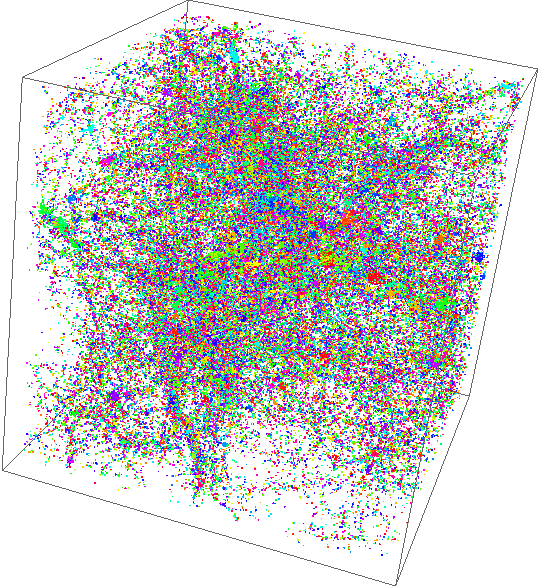
\includegraphics[width=4cm]{figures/cubemock.png}};
        \node[visible on=<5->]
            at ($ (current page.north west) + (10cm, -7cm) $)
            {\includegraphics[width=4cm]{figures/galaxy_mock.jpg}};
        \draw[line width=1pt, visible on=<4->]
            ($ (current page.north west) + (3.3cm, -2.45cm) $) --
            ($ (current page.north west) + (8.2cm, -0.9cm) $);
        \draw[line width=1pt, visible on=<4->]
            ($ (current page.north west) + (3.35cm, -2.75cm) $) --
            ($ (current page.north west) + (8cm, -3.8cm) $);
        \draw[line width=1pt, visible on=<5->]
            ($ (current page.north west) + (9cm, -3cm) $) --
            ($ (current page.north west) + (8cm, -5.45cm) $);
        \draw[line width=1pt, visible on=<5->]
            ($ (current page.north west) + (9cm, -3cm) $) --
            ($ (current page.north west) + (12cm, -5.45cm) $);
    \end{tikzpicture}
    \begin{columns}
        \begin{column}{0.64\textwidth}
            \vspace{3cm}
            \begin{minipage}[c][0.4\textheight][c]{\linewidth}
                \begin{block}{HOD or SAM}
                    \begin{itemize}
                        \item<1-> HOD (Halo Occupation Distribution):
                            populate dark matter halos with galaxies of fixed
                            properties
                        \item<2-> SAM (Semi Analytical Models): populate dark
                            matter halos with galaxies following physical
                            recipes in the code
                    \end{itemize}
                \end{block}
            \end{minipage}
        \end{column}
        \begin{column}{0.5\textwidth}
        \end{column}
    \end{columns}
\end{frame}

\subsection{Observational constraints}
\begin{frame}
    \begin{minipage}[c][0.4\textheight][c]{\linewidth}
        \vspace{1cm}
        \begin{tikzpicture}[
                mindmap,
                concept color=blue!60!white,
                text=white,
            ]
            \node[concept] (initial){%
                \begin{tikzpicture}[scale=0.5]
                    \draw[
                        domain=0:6,
                        smooth,
                        variable=\x,
                        blue,
                        samples=500,
                        line width=1pt,
                        label={0.5}{$\lambda_0$},
                    ]
                    plot ({\x}, {sin(10*\x r)});
                \end{tikzpicture}%
            }
            child[grow=right, visible on=<2->, concept
            color=blue!50!red!60!white, level distance=4.5cm] {%
                node[concept] (cosmo){%
                    
\begin{tikzpicture}[scale=0.3]
                        \draw[
                            domain=0:6,
                            smooth,
                            variable=\x,
                            blue!50!red,
                            samples=500,
                            line width=1pt,
                        ]
                        plot ({\x}, {sin(5*\x r)});
                    \end{tikzpicture}
                }
                child[visible on=<3->, concept color=red!60!white] {%
                    node[concept] (peculiar){%
                        
\begin{tikzpicture}[scale=0.2]
                            \draw[
                                domain=0:6,
                                smooth,
                                variable=\x,
                                red,
                                samples=500,
                                line width=1pt,
                            ]
                            plot ({\x}, {sin(\x r)});
                        \end{tikzpicture}
                    }
                }
            };
            \node[below, text=blue, visible on=<1->] at (initial)
            {Emitted\\$\lambda_0$};
            \node[below, text=blue!50!red, visible on=<2->] at (cosmo) {%
                Expansion\\$\left(1+z_{\cos}\right) \lambda_0$
            };
            \node[below, text=red, visible on=<3->] at (peculiar) {%
                Peculiar velocity\\
                $\left(1+z_\mathrm{pec}\right)\left(1+z_{\cos}\right) \lambda_0$
            };
        \end{tikzpicture}
    \end{minipage}
    \begin{minipage}[c][0.4\textheight][c]{\linewidth}
        \begin{block}{Observational effects}
            \begin{minipage}{0.59\linewidth}
                \begin{itemize}
                    \item<1-> Redshift distortions (Fingers-of-God)
                    \item<4-> K-corrections
                    \item<5-> Systematic errors
                \end{itemize}
            \end{minipage}
            \begin{minipage}{0.39\linewidth}
                \centering
                \includegraphics[width=\linewidth]{RS.pdf}\\
                \scriptsize Redshift space
            \end{minipage}
        \end{block}
    \end{minipage}
\end{frame}

\subsection{Galaxy samples}
\begin{frame}
    \begin{columns}
        \begin{column}{0.5\textwidth}
            \begin{minipage}[c][\textheight][c]{\linewidth}
                \begin{block}{Galaxy sub-samples}
                    \begin{itemize}
                        \item<1-> Realistic flux limited galaxy sample
                            (galaxies not sufficiently bright are not
                            observables)
                        \item<2-> Corrections for missing galaxies imprecise
                        \item<3-> Doubly complete samples don't need
                            corrections for missing galaxies
                        \item<4-> Divide the flux limited sample into complete
                            sub-samples
                    \end{itemize}
                \end{block}
            \end{minipage}
        \end{column}
        \begin{column}{0.5\textwidth}
            \begin{minipage}[c][\textheight][c]{\linewidth}
                \includegraphics[width=\linewidth]{subsamples.png}
            \end{minipage}
        \end{column}
    \end{columns}
\end{frame}

% vim: set tw=79:
